\chapter{Cells Cooperate to Build a Body}

\begin{kaichang}
Remember your last small injury: perhaps a cut while sharpening a pencil or a scraped knee. It bled and stung; you put on a bandage. A few days later, tender pink skin grew from the edges. Later still, the scab lifted and fell away, leaving barely a trace.

Consider this seriously: \textbf{how did the wound know a piece was missing, how much to replace, and when to stop?} No engineer directed the work or posted a blueprint nearby. Too little repair leaves a hole; too much makes a lump. Yet usually it stops in just the right place.

Write your guess. We will return to the wound at the end. The answer leads to a much larger question: why are trillions of cells willing---no, \emph{able}---to cooperate into a person?
\end{kaichang}

\section{Phenomena: A Wound in Slow Motion}

Leave molecules and cells aside and watch what is visible.

Within minutes, blood thickens and clots: bleeding stops. Over the next day or two, the surrounding skin becomes red, warm, slightly swollen, and painful, hotter to touch than nearby skin. Then soft, red, grainy granulation tissue grows beneath the wound, filling the hollow. Meanwhile, skin at the edges crawls inward to cover the surface. Finally, the scab falls away, revealing paler skin. A deep wound leaves a scar that may soften and fade over subsequent months.

\textbf{Translator safety note:} This is a simplified healing description, not a reason to ignore worsening redness, swelling, pain, pus, fever, or a serious wound. Seek medical advice for concerning symptoms; do not deliberately injure skin for observation. See \href{https://www.nhs.uk/conditions/cuts-and-grazes/}{NHS cuts-and-grazes guidance}.

Ordinary events tell the same story: the grime rubbed off during bathing contains many shed epidermal cells; clipped nails regrow over weeks; sunburned skin peels; mouth ulcers hurt for days and heal. \textbf{Your body is not a finished, unchanging statue but a construction site continually replacing old materials}. Injury merely accelerates and concentrates the work so we can see it.

\begin{shiyan}
\textbf{Give Your Nail a Measuring Gauge}

Materials: a fine-tipped washable colored pen, a millimeter ruler, and a calendar or phone notes.

Procedure: choose a thumbnail and draw a thin reference line on the nail near its base, beside the crescent where nail meets skin. Record the date. Every seven days, measure the distance from the line to the skin at the nail's base. Continue for three to four weeks.

Observations: is weekly growth similar? Calculate average millimeters per day. Why does the reference line itself not widen? Hint: is the already-grown nail still made of living cells?

Safety: mark only intact nail, not broken skin. Never carve a mark with a knife. Nails grow about \ud{3}{mm} monthly on average, varying greatly by person and finger; faster or slower measurements are normal.
\end{shiyan}

\section{Particles: Who Repairs the City?}

Zoom to the wound edge, as busy as an accident site.

First come \textbf{platelets}, cell fragments in blood. Contact with damaged vessel walls activates them to change shape and aggregate, plugging gaps like bags of quick-setting cement. Clotting factors simultaneously initiate a chain reaction that cuts soluble fibrinogen into fibrin, weaving a net that traps blood cells. This forms much of the scab, applying Chapter 49's enzyme-cascade principles.

Several resident repair teams follow. Immune cells remove bacteria and dead tissue; their recognition, responses, and memory are saved for Chapter 61. \textbf{Fibroblasts} secrete collagen and other matrix materials to fill the gap while pulling its edges inward. Edge \textbf{epithelial cells} change shape, loosen their connections, and spread toward the center like flattened palms, dividing as they migrate. Once the surface is covered, they reform layers and keratinize to restore the skin barrier. New capillaries grow into granulation tissue like water pipes, delivering materials and oxygen.

Notice: platelets, epithelial cells, fibroblasts, and vascular endothelial cells \textbf{look different and work differently, yet all belong to you}. Chapter 57 described the nucleus, mitochondria, and cytoskeleton inside every cell; Chapter 58 explained how signals and receptors convey outside commands. But neither settled why cells with the same DNA become epithelium in one place and muscle in another.

\section{Rules: One Manual, Different Pages}

DNA in almost every cell nucleus is identical, inherited as one fertilized egg became two cells, then four. The difference is not the manual's contents but \textbf{which pages each cell type opens}. This is \textbf{cell differentiation}: descendants gradually choose different gene-expression patterns and career paths.

Think of DNA as a library with tens of thousands of recipes. Epithelial cells borrow books on making keratin and packing tightly; muscle cells borrow actin and myosin, Chapter 48's contraction machinery; neurons borrow ion-channel and neurotransmitter recipes. Transcription factors control access by recognizing DNA switch sequences and activating or silencing nearby genes. These factors in turn respond to neighbors, matrix stiffness, and hormone concentrations, connecting to Chapter 58's signaling pathways.

Differentiation usually settles step by step through progressively narrowing junctions:

\begin{center}
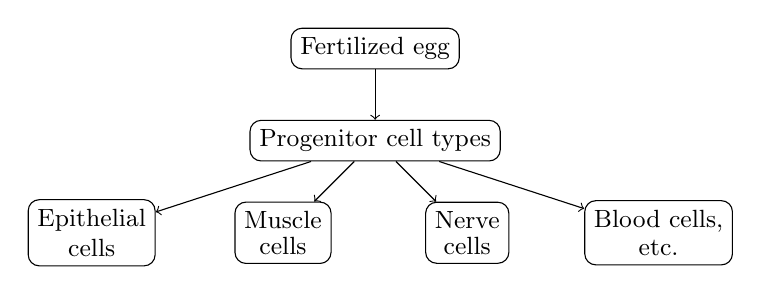
\begin{tikzpicture}[scale=0.9, every node/.style={font=\small}]
\node[draw, rounded corners] (z) at (0,0) {Fertilized egg};
\node[draw, rounded corners] (s) at (0,-1.3) {Progenitor cell types};
\node[draw, rounded corners] (a) at (-4,-2.6) {\shortstack{Epithelial\\cells}};
\node[draw, rounded corners] (b) at (-1.3,-2.6) {\shortstack{Muscle\\cells}};
\node[draw, rounded corners] (c) at (1.3,-2.6) {\shortstack{Nerve\\cells}};
\node[draw, rounded corners] (d) at (4,-2.6) {\shortstack{Blood cells,\\etc.}};
\draw[->] (z) -- (s);
\draw[->] (s) -- (a);
\draw[->] (s) -- (b);
\draw[->] (s) -- (c);
\draw[->] (s) -- (d);
\end{tikzpicture}
\end{center}

This representation aids thought: real differentiation narrows through many intermediate states, not one complete branching event.

\begin{zhengju}
Does differentiation close unused pages or tear them out? This dominated mid-twentieth-century developmental biology. Gene loss would make fully differentiated cells unable to return; expression shutdown would leave the full manual in the nucleus.

In 1962, the British scientist Gurdon performed a decisive test. He took nuclei from fully differentiated African clawed frog intestinal epithelial cells, specialized for digestion and absorption, and transplanted them into eggs whose nuclei had been removed. Some developed into normal tadpoles and even fertile adult frogs. Earlier nuclear transfers by Briggs and King using embryonic nuclei had mixed results, leading many to think advanced differentiation irreversible. Gurdon's result showed that \textbf{the intestinal nucleus had lost none of the instructions}: the entire frog-building manual remained, largely switched off, and egg cytoplasm could reset it.

In 2006, Shinya Yamanaka went further: four transcription factors, without an egg, rewound adult mouse skin cells into an embryonic-stem-cell-like state, induced pluripotent stem cells or iPS cells. Gurdon and Yamanaka shared the 2012 Nobel Prize in Physiology or Medicine. Notice the evidence chain: a falsifiable question, a decisive experiment, doubt and revision, then mechanisms resolved into particular molecules. That is how scientists know.
\end{zhengju}

\section{Four Building Materials: Tissues}

Differentiation produces hundreds of cell types. Structurally similar, functionally related cells and their secreted materials form a \textbf{tissue}. Animal tissues are traditionally grouped into four classes, a human classification much simpler than actual cell diversity.

\begin{itemize}[itemsep=2pt]
\item \textbf{Epithelial tissue:} outer walls and inner linings, including epidermis, digestive-tract lining, and alveolar walls. Closely locked cells have outward- and inward-facing sides and perform barrier, absorption, and secretion functions. At the front line of wear, they renew fastest.
\item \textbf{Connective tissue:} filling, connection, and support, including blood, fat, cartilage, bone, and tendons. It has relatively few cells and much between them. Bone is hard mainly because its secreted material is hard, not its cells.
\item \textbf{Muscle tissue:} contraction specialists. Skeletal muscle follows your commands, heart muscle works lifelong, and smooth muscle moves food and adjusts vessel diameter. Chapter 48 described actin--myosin sliding.
\item \textbf{Nervous tissue:} information highways. Neurons' long processes and electrochemical signals form a body-wide network; Chapter 58's neurotransmitters are its message parcels.
\end{itemize}

Give an overlooked participant its due: the \textbf{extracellular matrix}. Textbook cells often appear as crowded spheres with blank spaces between. Real cells sit in secreted gels and cables: collagen provides tensile strength through Chapter 48's triple helices, elastin supplies recoil, and water-binding proteoglycans provide compression-resistant cushions. Skin toughness, cartilage cushioning, and tendon strength depend mainly on these extracellular materials.

More importantly, matrix is \emph{not} inert filler. Integrin proteins span the cell membrane, gripping extracellular matrix on one side and Chapter 57's cytoskeleton on the other. Cells thus feel stiffness and tension and adjust division, movement, and differentiation. Stem cells on soft matrix tend toward neural fates; on stiff matrix, toward bone. Fibroblasts grip collagen and contract to draw wound edges together. Matrix composition and mechanics also change with age and disease, contributing to sagging skin and hardened atherosclerotic plaques.

\section{The Cooperation Pact: Renewal, Reserves, and Exit}

A society of trillions fears two things: no replacements and members refusing to leave. Multicellular bodies address them with two rules.

First, \textbf{continuous renewal}. Billions of epidermal cells shed daily; the intestinal lining is replaced every three to five days; red cells live about 120 days before the spleen recycles them. Replacements come from tissue \textbf{stem cells}: one daughter stays a stem cell while the other differentiates into new labor. Bone-marrow hematopoietic stem cells continually produce red cells, white cells, and platelets. Stem cells in intestinal crypts renew the surface within days, while the epidermal basal layer holds another reserve.

Second, \textbf{programmed cell death}, called apoptosis. Frightening as it sounds, it sustains cooperation. Internal damage detectors, advanced versions of Chapter 48's protein quality control, detect irreparable DNA damage or receive a signal that a cell is surplus. They initiate self-destruction: DNA is cut, the cell shrinks into fragments, and neighbors or immune cells quietly consume them without leakage or inflammation. This differs from accidental necrosis, where a ruptured cell spills its contents and provokes inflammation.

Too little apoptosis can mean cancer; too much, tissue wasting. It also builds: embryonic fingers start connected by webbing, and planned death between them separates the digits. A tadpole's tail disappears during metamorphosis through apoptosis, not simply by falling off.

\begin{qiaoliang}
How many cells change shifts? An adult has an estimated $3.7\times 10^{13}$ cells, thirty-seven trillion, though methods can differ severalfold. Blood and intestine renew especially rapidly: about $2\times 10^{11}$ new red cells daily. Convert this:
\[
\frac{2\times 10^{11}}{24\times 3600\ \text{seconds}} \approx 2\times 10^{6}\ \text{cells/second}
\]
Each second you read this, roughly \textbf{two million red blood cells} are born in bone marrow, while about as many expired cells are recycled in the spleen. Blood, intestine, and skin together replace about $3\times 10^{11}$ cells daily, less than one percent of the total. That sounds small, but over a year it replaces a substantial part of body-cell mass. Aging partly reflects declining precision in this shift-changing system.
\end{qiaoliang}

A tiny worm exposed programmed death's precision.

\begin{zhengju}
Caenorhabditis elegans is a transparent worm about \ud{1}{mm} long, with only 959 adult somatic cells, few enough to number and follow individually. In the 1970s and 1980s, Sulston and colleagues watched every division and cell fate from the fertilized egg and drew a complete lineage. They found an astonishing rule: development produces 1090 cells, exactly 131 of which die at fixed times and locations in every worm.

Such regular death cannot be accidental. Horvitz identified key genes including ced-3, ced-4, and ced-9. With ced-3 inactive, all 131 cells survive: death is an actively executed genetic program. Related genes later appeared across animals, including humans, with defects linked to cancer and neurodegeneration. Brenner, Horvitz, and Sulston received the 2002 Nobel Prize. A transparent worm established the counterintuitive fact that cellular self-destruction is part of development.
\end{zhengju}

\section{When Cooperation Fails: Cancer as Evolution}

We can now answer why cells cooperate: \textbf{cooperation is an evolutionary result, not a cellular virtue}.

Multicellular life evolved independently many times. Choanoflagellates, animals' closest living single-celled relatives, already have many adhesion and communication proteins, suggesting the cooperation toolkit preceded multicellularity. Once cells share a genome and their genes pass on only when the whole group survives, natural selection favors limits on division, responsiveness to signals, and self-destruction when needed. Your body is fundamentally a cooperation system shaped over billions of years.

But cheaters constantly threaten it. A cell may accumulate mutations that unleash division and disable apoptosis, abandoning the pact to multiply: a tumor. Chapter 58 showed tampered growth signals; here, \textbf{a tumor is a small evolutionary arena}. Divisions generate mutations, while immunity, oxygen shortage, and drugs impose selection. Descendants best at immune escape or drug resistance survive and expand. Chemotherapy may work initially then fail through the same logic as bacterial resistance in Chapter 62: killing sensitive cells clears space for resistant variants.

This perspective also presents Peto's paradox. Elephants have about a hundred times more cells than humans and long lives. If every division risks error, they should have much higher cancer risk, yet do not. Research suggests dozens of p53 tumor-suppressor copies in elephant genomes versus two in humans, enforcing apoptosis after DNA damage. Natural selection strengthened policing in large animals. Details remain under study, but anticancer mechanisms themselves are evolutionary products.

\section{Limits: Where the Picture Distorts}

Several simplifications need boundaries.

First, the four tissue classes come from microscopy two centuries ago. Modern single-cell sequencing reveals continuous spectra rather than tidy drawers. Macrophages differ greatly among organs and continually respond to environment. The four classes remain useful maps, not rigid boxes.

Second, one-way differentiation is being revised. Gurdon's work and iPS technology show resetting is possible, and differentiated cells in organs such as the liver can turn back after injury to replenish other types. But laboratory plasticity is not ordinary life: most human differentiation is stable, and scars remain because repair is not always perfect regeneration.

Third, this wound-healing account describes small skin wounds. Serious burns or chronic wounds such as diabetic foot ulcers can stall; spinal and brain neurons hardly regenerate. Repair varies enormously among tissues and species. Salamanders regrow whole limbs while we make scars, for reasons not fully understood.

\begin{wuqu}
``Differentiation discards unused genes, leaving each cell only the DNA it needs.'' Counterexample one: individual differentiated cells from dispersed carrot-root phloem can grow into complete flowering carrots in culture, now routine in plant propagation. Counterexample two: Gurdon's nuclear transfers and Dolly the sheep, whose mammary-cell nucleus directed a whole sheep. Gene loss would make these impossible. \textbf{Differentiation changes expression switches, not which genes exist}. This distinction is not wordplay: cloning and regenerative medicine depend on the manual still being present.
\end{wuqu}

\section{Back to the Wound}

Take the opening question apart.

How does the wound know something is missing? In intact epithelium, close cell contact itself inhibits division. A gap removes contact and tension from edge cells; platelet growth factors, Chapter 58's signals, add stimulation. Released brakes plus accelerator start division and inward migration.

How does it know how much to replace? When opposing epithelial fronts meet, contact returns, restoring brakes and stopping division and migration. Fibroblasts remodel underlying granulation tissue into stronger collagen, while surplus new vessels regress through apoptosis.

How does it know when to stop? It does not know: feedback makes the command disappear when the task is complete. Like an air conditioner, sensors, controllers, and effectors form a closed loop without understanding temperature. Next chapter shows such loops maintaining temperature, glucose, and blood pressure.

The scar records quick repair rather than exact reconstruction: dense, disordered collagen lacks hair follicles and sweat glands. Evolution favored speed; rapidly sealing wounds against infection mattered more to wild ancestors than appearance.

\section{Going Deeper: From Repair to Tissue Engineering}

Understanding cooperation lets humans intervene. Hematopoietic stem-cell transplantation, or bone-marrow transplantation, rebuilds a patient's blood system with healthy donor stem cells and is an established leukemia treatment. It works because stem cells self-renew and make every blood-cell type. Extensive burns can receive cultured autologous epidermal grafts: a small skin sample expands in the laboratory into sheets for the wound. Scientists also use 3D printing and matrix-like scaffolds to attempt more complex tissues.

But a caution: many marketed stem-cell beauty and anti-aging procedures have evidence far below these established treatments. Most lack rigorous controlled trials, and some risk inducing tumors. Stem cells promote division, after all, and uncontrolled division is not far away. Always ask where evidence comes from and whether doses and risks are clear.

\textbf{Translator safety note:} Do not treat a clinic's stem-cell or regenerative label as proof of safety or effectiveness. Discuss treatment with a qualified specialist and check its authorization for the intended use. See the \href{https://www.fda.gov/vaccines-blood-biologics/consumers-biologics/important-patient-and-consumer-information-about-regenerative-medicine-therapies}{FDA warning about unapproved regenerative therapies}.

Regeneration is another frontier. Why can salamanders regenerate heart and spinal tissue while humans cannot? Differences in matrix, inflammation, and differentiation may hold the answer. Finding a safe way to rewind human tissue would combine this chapter's rules in a major application.

All of this---wound repair, blood renewal, temperature maintenance---requires trillions of cells to operate in a shared chemical environment. What if glucose rises, temperature falls, or pH shifts slightly? How does the body keep these variables in narrow ranges? That is the next chapter: homeostasis.

\begin{tiaozhan}
\textbf{How Many Divisions Make a Person?} (optional)

Assume $3.7\times 10^{13}$ body cells, all descended from a fertilized egg. If each generation doubles the count, $n$ generations satisfy $2^n \approx 3.7\times 10^{13}$. Taking base-two logarithms:
\[
n = \log_2(3.7\times 10^{13}) \approx 45
\]
Only about 45 generations! That is exponential growth. Reality is more complex: many cells undergo planned apoptosis, as with the worm's 131; tissues divide different numbers of times; neurons largely stop dividing after birth, while fat-cell counts change with weight. Thus 45 is a rough lower-bound estimate, useful for grasping where $10^{13}$ cells come from, not an exact answer.
\end{tiaozhan}

\section*{Practice}

\begin{sikaoti}
\item Draw a wound material-flow map with boxes for scab, granulation tissue, new epithelium, and scar. Label arrows with which participants---platelets, fibroblasts, epithelial cells, and vessels---deliver which materials where. Focus on the process, not cell shapes.
\item Epithelial and nerve cells have nearly identical DNA but very different functions. Explain differentiation as borrowing from different library shelves. Use Gurdon's transfers to show why the experiment supports closed books rather than torn-out pages.
\item Why do migrating epithelial cells stop when they meet centrally? Express contact inhibition as a negative-feedback loop: stimulus → response → stimulus disappears. Give a similar everyday example.
\item Apoptosis sculpts fingers and removes precancerous cells. Refute the claim that cell death is always bad and should be prevented with drugs. Then explain why more apoptosis is not always better either.
\item With a red-cell lifespan of about 120 days and $2\times 10^{11}$ new cells daily, estimate the total red-cell population by multiplication and express it in scientific notation.
\item Peto's paradox concerns animals with many cells and long lives that do not have the expected high cancer risk. Propose an evolutionary explanation for elephants and describe evidence that could test it.
\end{sikaoti}
